\section{Teil}
beinhaltet folgende Foliensätze:

\begin{itemize}
    \item Teil 5: Digitaler Zwilling

\end{itemize}

% subsection
%-------------------------------------------------------------------------------------------
\subsection{Erklären Sie in eigenen Worten den Begriff Digitaler Zwilling!}
Ein Digitaler Zwilling ist ein virtuelles Abbild eines realen Objekts oder Systems. 
Er besteht aus dem realen Objekt, dem digitalen Modell und den Daten, die beide miteinander verbinden, um das reale Objekt in Echtzeit oder für Simulationen abzubilden.


% subsection
%-------------------------------------------------------------------------------------------
\subsection{Was ist ein Digitaler Schatten?}
Ein Digitaler Schatten beschreibt die Echtzeitdarstellung von Betriebs-, Zustands- oder Prozessdaten eines realen Objekts oder Systems, ohne dass ein vollständiges Modell vorliegt. 

Im Gegensatz zum Digitalen Zwilling umfasst er kein vollständiges Modell, sondern nur die kontinuierlich erfassten Daten, die den aktuellen Zustand des Systems widerspiegeln. 

Diese Daten ermöglichen die Überwachung und Analyse des realen Objekts ohne Modellierung des gesamten Verhaltens.

\begin{figure}[H]
    \centering
    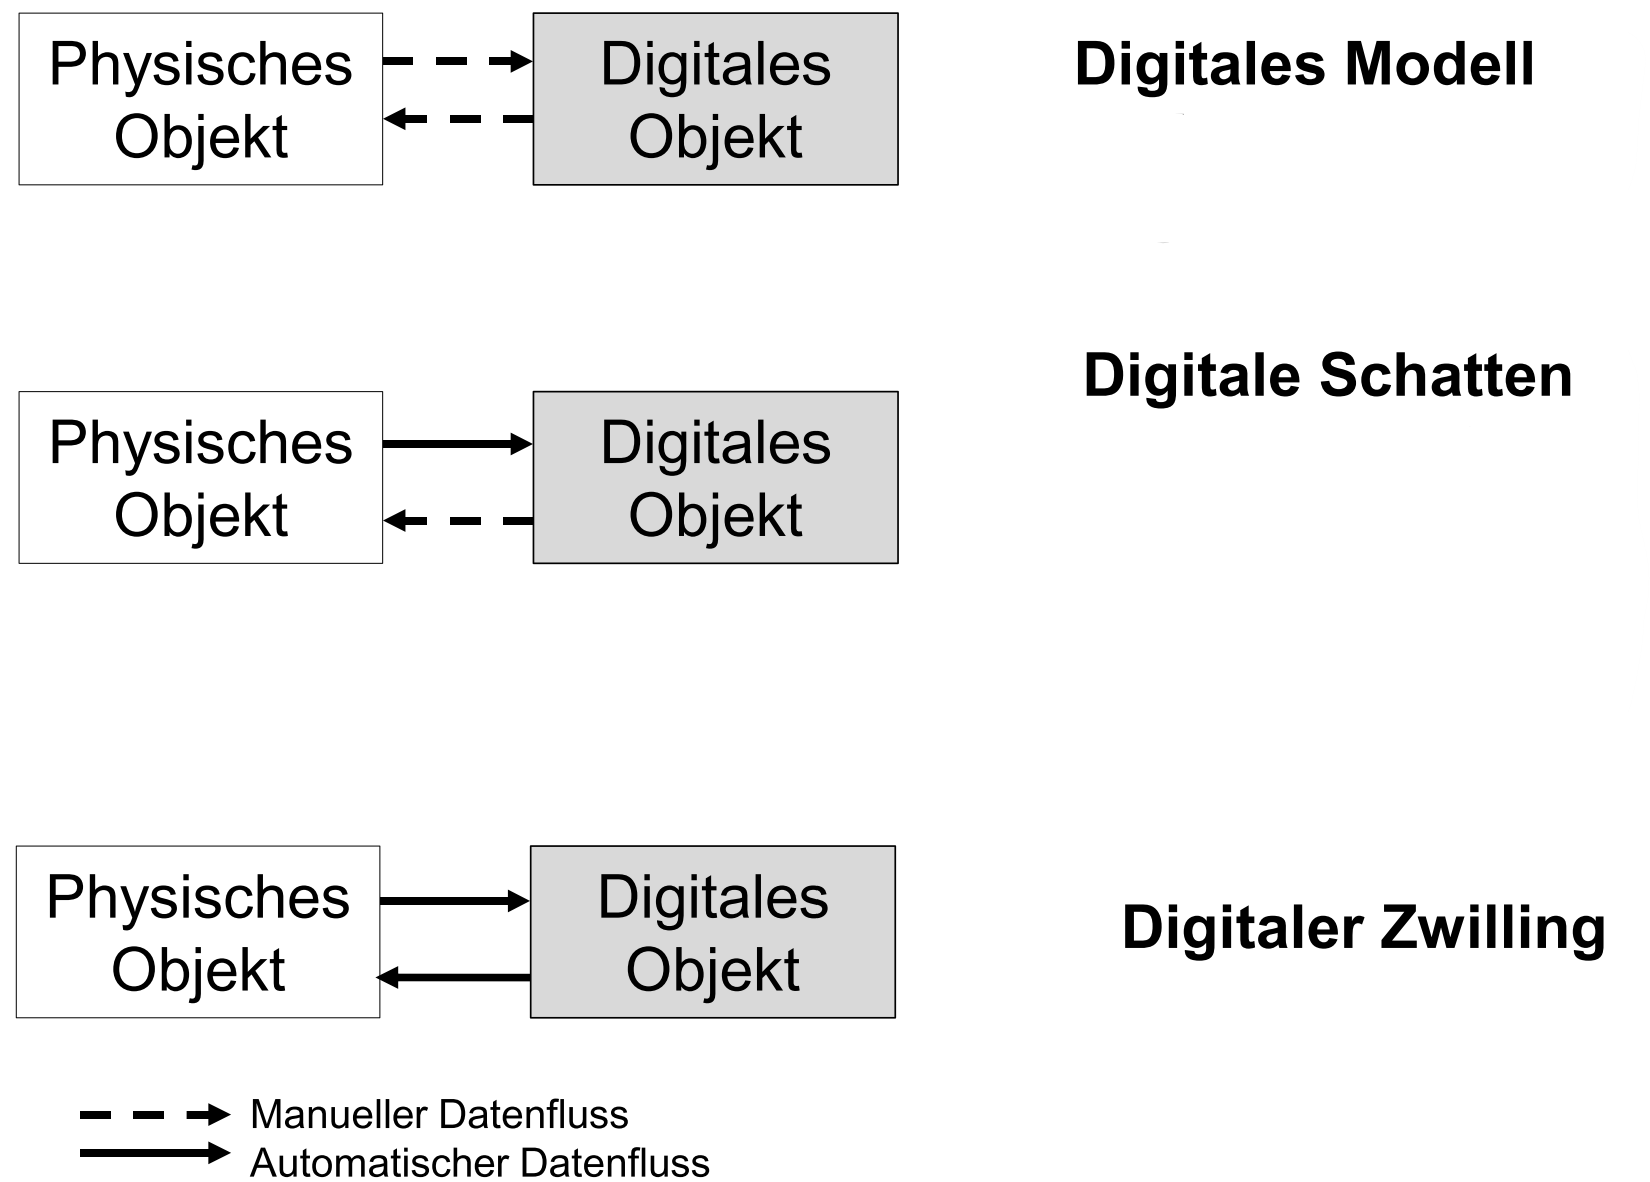
\includegraphics[width=0.6\linewidth]{Bilder/Teil5_Begriffe.png}
    \caption{Begriffe Digitales Modell, Digitaler Schatten, Digitaler Zwilling}
\end{figure}

% subsection
%-------------------------------------------------------------------------------------------
\subsection{Was bedeutet Functional Mock-Up Interface?}
Das Functional Mock-Up Interface (FMI) ist eine standardisierte Schnittstelle, die den Austausch und die Integration von Simulationsmodellen zwischen verschiedenen Softwareumgebungen ermöglicht. 

Es erlaubt die Kosimulation, bei der Modelle in verschiedenen Tools gemeinsam ausgeführt werden, ohne dass das Modell in jedem Tool neu erstellt werden muss.